\section{Encoding of Correlated Sources and Slepian-Wolf Theorem}
\subsection{Some Definitions}
%
\begin{tcolorbox}[boxrule=0pt,frame hidden,sharp corners,enhanced, opacityback=0, borderline west={2pt}{0pt}{red}]
\begin{defn} \textbf{($(2^{nR_1}, 2^{nR_2}),n)$ distributed source code)} A ($(2^{nR_1}, 2^{nR_2}),n)$ distributed source code for the joint source $(X,Y)$ consists of two encoder maps,
%
\begin{eqnarray}
f_1 : \mathcal{X}^n \rightarrow \{1,2,...,2^{nR_1}\}, \\
f_2 : \mathcal{Y}^n \rightarrow \{1,2,...,2^{nR_2}\},
\end{eqnarray}
%
and a decoder map,
%
\begin{eqnarray}
 g : \{1,2,...,2^{nR_1}\} \times \{1,2,...,2^{nR_2}\} \rightarrow  \mathcal{X}^n \times \mathcal{Y}^n.
\end{eqnarray}
%
Here $f_1(X^n)$ is the index corresponding to $X^n$ and $f_2(Y^n)$ is the index corresponding to $Y^n$. 
\end{defn}
\end{tcolorbox}
%
\begin{tcolorbox}[boxrule=0pt,frame hidden,sharp corners,enhanced, opacityback=0, borderline west={2pt}{0pt}{red}]
\begin{defn} \textbf{(Probability of Error)} The probability of error for a distributed source code is defined as
%
\begin{eqnarray}
    P_e^{(n)} = P(g(f_1(X^n), f_2(X^n)) \neq (X^n, Y^n)).
\end{eqnarray}
%
\end{defn}
\end{tcolorbox}
%
\begin{tcolorbox}[boxrule=0pt,frame hidden,sharp corners,enhanced, opacityback=0, borderline west={2pt}{0pt}{red}]
\begin{defn} \textbf{(A rate pair $(R_1, R_2)$)} A rate pair $(R1, R2)$ is said to be achievable for a distributed
source if there exists a sequence of $(2^{nR_1}, 2^{nR_2}),n)$ distributed source codes with the probability of error $P_e^{(n)} \rightarrow 0$. The achievable rate region is
the closure of the set of achievable rates.
\end{defn}
\end{tcolorbox}
%
%%%%%%%%%%%%%%%%%%%%%%%%%%%%%
\subsection{Slepain-Wolf Theorem}
%
\begin{tcolorbox}[boxrule=0pt,frame hidden,sharp corners,enhanced, opacityback=0, borderline west={2pt}{0pt}{blue}]
\begin{thm} 
For the distributed source coding problem for the source $(X,Y)$ drawn i.i.d. $\sim p(x,y)$, the achievable rate region is given by
%
\begin{eqnarray}
  R_1 &\geq& H(X|Y), \\
  R_2 &\geq& H(Y|X), \\
  R_1+R_2 &\geq& H(X,Y).
\end{eqnarray}
%
\end{thm}
\end{tcolorbox}
%
Let us demonstrate the result with an example. Consider $(X,Y)$ have the joint probability mass function $p(x,y)$:
%
%
\begin{eqnarray}
   \begin{tabular}{|c|c|c|c|}
        \hline
        \backslashbox{$X$}{$Y$} & 0 & 1 \\
       \hline
        0 & $\frac{1}{3}$ & $\frac{1}{3}$ \\
        \hline
        1 & 0 & $\frac{1}{3}$ \\
        \hline
    \end{tabular}
\end{eqnarray}
%
In this case, if we want to transmit the sources independently, it will require $2$ bits. Let us calculate how many bits are necessary for Slepain-Wolf encoding. Now,
%
\begin{eqnarray}
    H(X) = -\sum_{x} p(x)\log p(x) = -\frac{1}{3}\log\frac{1}{3}-\frac{2}{3}\log\frac{2}{3} = 0.918 \mbox{ bits},
\end{eqnarray}
%
and
%
\begin{eqnarray}
H(Y|X) = \sum_{x} p(X=x)H(Y|X=x) = \frac{1}{3}H(1,0)+\frac{2}{3}H(\frac{1}{2},\frac{1}{2}) = 0.667 \mbox{ bits}.
\end{eqnarray}
%
Hence, for Slepain-Wolf encoding, we only need 1.584 bits.
%%%%%%%%%%%%%%%%%%%%%%%%%%%%%%%%%%%%%%
\subsection{Achievability of the Slepian-Wolf Theorem}
\subsection{Converse of the Slepian-Wolf Theorem}
%%%%%%%%%%%%%%%%%%%%%%%%%%%%%%%%%%%%%%%
\subsection{Slepian-Wolf Theorem for Many Sources}
The Slepain-Wolf theorem can be generalized to many sources. Therefore we can state the theorem as follows.
%
\begin{tcolorbox}[boxrule=0pt,frame hidden,sharp corners,enhanced, opacityback=0, borderline west={2pt}{0pt}{blue}]
\begin{thm} 
Let $(X_{1i},X_{2i},...,X_{mi})$ be i.i.d. $\sim p(x_1,x_2,...,x_m)$. Then the set of rate vectors achievable for distributed source coding with separate encoders and a common decoder is defined by
%
\begin{eqnarray}
    R(S) > H(X(S)|X(S^c))
\end{eqnarray}
%
for all $S \subseteq \{1,2,...,m\}$, where
%
\begin{eqnarray}
    R(S) = \sum_{i \in S} R_i
\end{eqnarray}
%
and $X(S) = \{X_j: j\in S\}$.
\end{thm}
\end{tcolorbox}
%
The rate region defined in the Slepian-Wolf theorem is shown in figure \ref{fig:SME).
%
\begin{figure}[h]
    \centering
    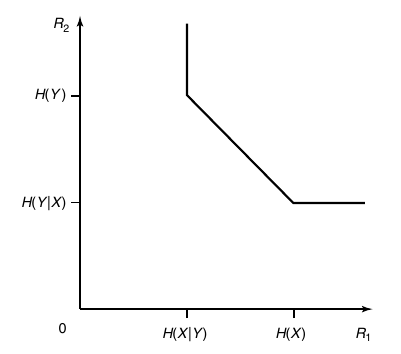
\includegraphics[scale=0.40]{Diagrams/SWE.png}
    \caption{Rate region for Slepian-Wolf encoding}
    \label{fig:SME}
\end{figure}
%